%\documentclass[handout,mathserif]{beamer}
%\usepackage{pgfpages}
%\pgfpagesuselayout{4 on 1}[a4paper, landscape, border shrink=5mm]
%\pgfpageslogicalpageoptions{1}{border code=\pgfusepath{stroke}}
%\pgfpageslogicalpageoptions{2}{border code=\pgfusepath{stroke}}
%\pgfpageslogicalpageoptions{3}{border code=\pgfusepath{stroke}}
%\pgfpageslogicalpageoptions{4}{border code=\pgfusepath{stroke}}
\documentclass{beamer}
%\usetheme{nesl}  % Now it's a beamer presentation with the NESL theme!
\usetheme{Warsaw}
\usepackage{tikz}
\usetikzlibrary{shapes,arrows}
\usepackage{url}
\usepackage{movie15}
\usepackage{verbatim}
\usefonttheme{serif}
\setbeamercolor{headcolour}{parent=palette secondary} 

\setbeamertemplate{headline} 
{% 
\begin{beamercolorbox}[wd=\paperwidth,ht=4.25ex,dp=2ex]{headcolour}% 
  \Tiny\insertsectionnavigationhorizontal{\textwidth}{}{} 
  \end{beamercolorbox}% 
  } 

% Make a new command that will make a new subsection and a frame with the same title
\newcommand{\fst}[2]{\subsection{#1}\frame{\frametitle{#1} #2}}

% Standard LaTeX stuff - note the optional abbreviated title being provided
\title[Development of WRF/GSI 4D-Var]{Recent development of WRF 4D-Var and \\GSI-based WRF 4D-Var}
\author[Zhang et al.]{Xin Zhang \and Xiang-Yu Huang}

\date{~\\\tiny{June 15, 2011}
~\\
~\\\tiny{NMC/CMA, Beijing,China}\\
  ~\\
  ~\\
  ~\\
 \tiny{NCAR is sponsored by the National Science Foundation}
}

\institute[NCAR Earth System Laboratory]{
% \url{xinzhang@ucar.edu} \\
   NCAR Earth System Laboratory \\
%  \url{ook@ucw.cz}\\
%  Charles University, Prague
}

% We want the NSF department logo
\logo{\includegraphics[height=.25in]{NSF_NESL.jpg}}


\begin{document}

% The title page
\frame{\titlepage}

%%%%%%%%%%%%%%%%%%%%%%%%%
\section{Introduction of 4D-Var}

\frame{
\frametitle{\small Observation System}
\begin{center}
\includegraphics[scale=0.25]{observation_system.png}
\end{center}
}

\frame{
\frametitle{\small Why data assimilation?}
\begin{itemize}
	\item Initial conditions \pause
	\item Observing system design, monitoring and assessment
\end{itemize}
}

\frame{
\frametitle{\small Forecast sensitivity to Observation}
\begin{center}
\includegraphics[scale=0.25]{FSO.png}
\end{center}
}

\frame{
\frametitle{\small Why data assimilation?}
\begin{itemize}
	\item Initial conditions
	\item Observing system design, monitoring and assessment
	\item Reanalysis \pause
	\item Calibration and validation
\end{itemize}
}

\frame{
\frametitle{\small Assimilation methods}
\begin{itemize}
	\item Empirical methods
	\begin{itemize}
		\item Successive Correction Method (SCM)
		\item Nudging
		\item Physical Initialization (PI), Latent Heating Nudging (LHN)	\pause
	\end{itemize}
	\item Statistical methods
		\begin{itemize}
		\item Optimal Interpolation (OI)
		\item 3-Dimensional VARiational data assimilation (3DVAR)
		\item \color{red}{4-Dimensional VARiational data assimilation (4DVAR)} \pause
	\end{itemize}
	\item Advanced methods
		\begin{itemize}
		\item Extended Kalman Filter (EKF)
		\item Ensemble Kalman Filter (EnFK) \pause
	\end{itemize}
\end{itemize}
}

\frame{
\frametitle{\small 4D-Var versus 3D-Var\\(Adopted from ECMWF training Course 2008)}
\begin{itemize}
	\item 4D-Var is comparing observations with background model fields at the correct time \pause
	\item 4D-Var can use observations from frequently reporting stations \pause
	\item The dynamics and physics of the forecast model is in an integral part of 4D-Var, so observations are used in a meteorologically more consistent way \pause
	\item 4D-Var combines observations at different times during the 4D-Var window in a way that reduces analysis error \pause
	\item 4D-Var propagates information horizontally and vertically in a meteorologically more consistent way
\end{itemize}
}

\section{Progress of upgraded WRF 4D-Var}

\frame{
\begin{center}
\large Part I \\
~\\
~\\
\large Progress and status of WRF 4D-Var V3.3
\end{center}
}

\subsection{Upgraded to WRF 4D-Var V3.3}

\frame{
\frametitle{\small Status of WRF 4D-Var V3.2}
\begin{itemize}
	\item WRF 4D-Var was firstly released in April, 2009 with V3.1. \pause
	\item WRF adjoint and tangent linear codes (WRFPLUS) were developed based on WRF V2.0.2 around 2005. \pause
	\item Multiple Program Multiple Data (MPMD) framework, needs 3 executables: WRFDA, WRFNL and WRFPLUS. \pause
	\item Simplified physical packages: surface drag, large scale condensation and a cumulus parameterization schemes. \pause
	\item Weak constraint with digital filter.
\end{itemize}
}

\frame{
\frametitle{\small Known issues of WRF 4D-Var V3.2}
\begin{itemize}
	\item Numerous bug fixes, upgrades and improvements in WRF model since 2005. V3.3 is released.\pause
	\item Particularly, WRF infrastructure changes invalid some interfaces in WRFPLUS, such as the boundary variables can not be read in anymore.\pause
	\item MPMD WRF 4D-Var is too complicate, most of the community users could not get it run without help. \pause
	\item Very high disk IO overhead associated with the number of processors.\pause
	\item Only runs good on IBM machines; unstable on other platforms and compilers.\pause
	\item 4D-Var support for Prepbufr and radiance bufr data is not clear. \pause
	\item Hard to do a complete adjoint check due to initial design of framework.
\end{itemize}
}

\frame{
\frametitle{\small WRFPLUS V3.3 Upgrades}
\begin{itemize}
   	\item WRF adjoint and tangent linear codes V3.3 based on the latest WRF V3.3. \pause
	\item Constructed interfaces through which other applications can call WRF adjoint and tangent linear model directly. \pause 
	\item Testing the code on various  platforms and compilers ( IBM, Linux, Mac : xlf, g95, pgi, intel, gfortran). \pause
	\item Capability to do tangent linear and adjoint test over any length of time window. \pause 
	\item WRFPLUS V3.3 can be used as a standalone tool or as a component in 4D-Var system.\pause
	\item Only serial run is support for V3.3 WRF 4D-Var.
\end{itemize}
}

\begin{frame}[fragile]
\frametitle{\small Sample Tangent Linear and Adjoint Check of WRFPLUS V3.3 }
\setbeamercolor{postit}{fg=black, bg=yellow}
\begin{beamerboxesrounded}[ lower=postit,shadow=true]{Tangent linear check:6 hours}
{\tiny
\begin{verbatim}
alpha_m=.1000E+00  coef=   0.98186174930325E+00  val_n= 0.3725210E+11  val_l= 0.3794027E+11
alpha_m=.1000E-01  coef=   0.99807498026522E+00  val_n= 0.3786723E+09  val_l= 0.3794027E+09
alpha_m=.1000E-02  coef=   0.99970559707666E+00  val_n= 0.3792910E+07  val_l= 0.3794027E+07
alpha_m=.1000E-03  coef=   0.99992019503144E+00  val_n= 0.3793724E+05  val_l= 0.3794027E+05
alpha_m=.1000E-04  coef=   0.10000447262220E+01  val_n= 0.3794196E+03  val_l= 0.3794027E+03
alpha_m=.1000E-05  coef=   0.99999981575068E+00  val_n= 0.3794026E+01  val_l= 0.3794027E+01
alpha_m=.1000E-06  coef=   0.99999998152933E+00  val_n= 0.3794027E-01  val_l= 0.3794027E-01
alpha_m=.1000E-07  coef=   0.99999990980017E+00  val_n= 0.3794026E-03  val_l= 0.3794027E-03
alpha_m=.1000E-08  coef=   0.99999956711797E+00  val_n= 0.3794025E-05  val_l= 0.3794027E-05
alpha_m=.1000E-09  coef=   0.10000030220656E+01  val_n= 0.3794038E-07  val_l= 0.3794027E-07
alpha_m=.1000E-10  coef=   0.99996176999678E+00  val_n= 0.3793882E-09  val_l= 0.3794027E-09
\end{verbatim}
}
\end{beamerboxesrounded}
\begin{beamerboxesrounded}[ lower=postit,shadow=true]{Adjoint check: 6 hours}
{\tiny
\begin{verbatim}
 ad_check: VAL_TL:    0.42476489986911E+11
 ad_check: VAL_AD:    0.42476489986912E+11
\end{verbatim}
}
\end{beamerboxesrounded}
\end{frame}

\begin{frame}[fragile]
\frametitle{\small Single executable 4D-Var}
WRFPLUS includes WRF NL, AD and TL model and they are used as subroutines in WRF 4D-Var V3.3, other than being called via shell scripts in V3.2.
~\\
~\\
\setbeamercolor{postit}{fg=black, bg=yellow}
\begin{beamerboxesrounded}[ lower=postit,shadow=true]{Nonlinear call}
\begin{verbatim}
old         call da_system ("da_run_wrf_nl.ksh")
new         call da_nl_model
\end{verbatim}
\end{beamerboxesrounded}
\begin{beamerboxesrounded}[ lower=postit,shadow=true]{Tangent linear call}
\begin{verbatim}
old         call da_system ("da_run_wrfplus_tl.ksh")
new         call da_tl_model
\end{verbatim}
\end{beamerboxesrounded}
\begin{beamerboxesrounded}[ lower=postit,shadow=true]{Adjoint call}
\begin{verbatim}
old         call da_system ("da_run_wrfplus_ad.ksh")
new         call da_ad_model
\end{verbatim}
\end{beamerboxesrounded}
\end{frame}

\begin{comment}
\begin{frame}[fragile]
\frametitle{\small Memory exchange}
The information (TL perturbation, adjoint forcing, basic states and gradient) is exchanged via linked lists.
~\\
~\\
\setbeamercolor{postit}{fg=black, bg=yellow}
\begin{beamerboxesrounded}[ lower=postit,shadow=true]{Read basic states}
\begin{verbatim}
call domain_clock_get( grid, current_timestr=timestr )
call da_read_basicstates ( xbx, grid, ... )
\end{verbatim}
\end{beamerboxesrounded}
\begin{beamerboxesrounded}[ lower=postit,shadow=true]{Save TL perturbation}
\begin{verbatim}
call push_tl_pert (timestr)
\end{verbatim}
\end{beamerboxesrounded}
\begin{beamerboxesrounded}[ lower=postit,shadow=true]{Save AD forcing}
\begin{verbatim}
call push_ad_forcing (timestr)
\end{verbatim}
\end{beamerboxesrounded}
\end{frame}
\end{comment}

\frame{
\frametitle{\small Parallel run mechanism of V3.2}
4D-Var is a sequential algorithm. However, the parallel WRF 4D-Var V3.2 was constructed on the Multiple Program Multiple Data mode, which has to split the total processors into 3 subsets for DA, NL and AD/TL. Lots of CPU time are wasted
\begin{center}
\includegraphics[scale=0.5]{mpmd_wrf4dvar}
\end{center}
}

\frame{
\frametitle{\small Parallel run using all processors with V3.3}
Benefit from the single executable framework, every CPU is working at any time. No IDLE any more.
\begin{center}
\includegraphics[scale=0.5]{single_exe_wrf4dvar}
\end{center}
}

\begin{comment}
\frame{
\frametitle{\small Performance improvement WRF 4DVar framework only}
\begin{itemize}
	\item 90\times60\times41, 60km, 6h window, 1h obs\_bin
	\item 27 iterations FGAT, NCAR bluefire (IBM P6)
\end{itemize}
\begin{center}
\includegraphics[scale=0.5]{small_case_performance}
\end{center}
}
\end{comment}

\frame{
\frametitle{\small Performance improvement WRF 4DVar framework only}
\begin{itemize}
	\item 270X180X41@20km,6h window, 1h obs\_bin, 10 iterations
	\item 10 iterations FGAT, NCAR bluefire (IBM P6)
\end{itemize}
\begin{center}
\includegraphics[scale=0.5]{big_case_performance}
\end{center}
}

\fst{\small Weak constraint with digital filter (enhanced)}{
\begin{tabular}{l p{2in}}
\includegraphics[scale=0.25]{jcdf_formular} \pause & \includegraphics[scale=0.25]{jcdf}
\end{tabular}
}

\frame{
\frametitle{\small Weak constraint with digital filter \\(domain averaged surface pressure variation) }
\begin{center}
\includegraphics[scale=0.25]{jcdf_ps}
\end{center}
}

\begin{comment}
\fst{\small Observations used by 4D-Var}{
\begin{itemize}
	\item Conventional observational data (little\_r, prepbufr)
	\item Radar radial velocity
	\item Radiance satellite data
\end{itemize}
\begin{center}
\includegraphics[scale=0.25]{obs_3dvar} \pause
\vspace {-13.61em} \includegraphics[scale=0.25]{obs_4dvar}
\end{center} 
}
\end{comment}

%%%%%%%%%%%%%%%%%%%%%%%%%

\fst{\small Single observation experiments}{
\begin{itemize}
	\item Initial time: $2000\_01\_25\_00:00:00$
	\item Ending time: $2000\_01\_25\_06:00:00$
	\item Observation: 500 mb Temperature at {\color{red}ending time} \\
	          $O-B=-1.168K$
	\item To investigate the difference at {\color{red}ending time} between the forecast from analysis and from background.
\end{itemize}
}

\frame{
\frametitle{\small Single observation experiments, LBC control is on}
\begin{columns}[c]
\column{5cm}
\includemovie[
  controls,poster={centerlbcjcdf.pdf},
  text={\large(Click to start the movie)\hspace*{400pt}}
]{6.0cm}{7.5cm}{centerlbcjcdf.mpeg}
\column[c]{3.5cm}
\begin{block}{Remarks}
\tiny{Forecasted 500mb T difference \\(DA forecast - reference forecast)}
\begin{itemize}
	\item {\color{red}$\star$} is the location of obs. at the ending time (6h).
	\item \tiny{JcDF is turned on}
	\item \tiny{LBC control is turned on}
	\item \tiny{Initial perturbation is on the upstream of the obs.}
	\item \tiny{Evolved perturbation at 6h hit the obs. location}
\end{itemize}
\end{block}
\end{columns}
}

\begin{comment}
\frame{
\frametitle{\small Single observation experiments, LBC control is off}
\begin{columns}[c]
\column{5cm}
\includemovie[
  controls,poster={centernolbcjcdf.pdf},
  text={\large(Click to start the movie)\hspace*{400pt}}
]{6.0cm}{7.5cm}{centernolbcjcdf.mpeg}
\column[c]{3.5cm}
\begin{block}{Remarks}
\tiny{Forecasted 500mb T difference \\(DA forecast - reference forecast)}
\begin{itemize}
	\item {\color{red}$\star$} is the location of obs. at the ending time (6h).
	\item \tiny{JcDF is turned on}
	\item \tiny{LBC control is  {\color{red}turned off}}
	\end{itemize}
\end{block}
\end{columns}
}
\end{comment}

\fst{\small Consider Lateral boundary condition as control variable}{
\begin{equation*}
J=J_b+J_o+J_c+\color{red}J_{lbc}
\end{equation*}
\begin{eqnarray*}
J_{lbc} & = & \frac{1}{2}(\mathbf{x}(t_k)-\mathbf{x}_b(t_k))^T\mathbf{B}^{-1}(\mathbf{x}(t_k)-\mathbf{x}_b(t_k))\\
& = & \frac{1}{2}\delta\mathbf{x}(t_k)^T\mathbf{B}^{-1}\delta\mathbf{x}({t_k})
\end{eqnarray*}
$J_{lbc}$ is the $J_b$ at the end of the assimilation window \\
lateral boundary control is obtained through
\begin{eqnarray*}
\frac {\partial{\delta{\mathbf{x}}_{lbc}}} {\partial{t}}=\frac{\delta\mathbf{x}(t_k)-\delta\mathbf{x}(t_0)}{t_k-t_0}
\end{eqnarray*}
}

\frame{
\frametitle{\small Single observation close to boundary}
To investigate the impact of including boundary condition in data assimilation, the 6h observation is close to boundary and downstream of the boundary, we expect that the analysis response at 0h should be in boundary condition other than initial condition.
}

\frame{
\frametitle{\small Single observation experiments, LBC control is on}
\begin{columns}[c]
\column{5cm}
\includemovie[
  controls,poster={boundarylbcjcdf.pdf},
  text={\large(Click to start the movie)\hspace*{400pt}}
]{6.0cm}{7.5cm}{boundarylbcjcdf.mpeg}
\column[c]{3.5cm}
\begin{block}{Remarks}
\tiny{Forecasted 500mb T difference \\(DA forecast - reference forecast)}
\begin{itemize}
	\item {\color{red}$\star$} is the location of obs. at the ending time (6h).
	\item \tiny{LBC control is {\color{red}turned on}}
	\item \tiny{Major initial perturbation is in LBC  other than inIC ( south boundary, invisible here)}
\end{itemize}
\end{block}
\end{columns}
}

\frame{
\frametitle{\small Single observation experiments, LBC control is off}
\begin{columns}[c]
\column{5cm}
\includemovie[
  controls,poster={boundarynolbcjcdf.pdf},
  text={\large(Click to start the movie)\hspace*{400pt}}
]{6.0cm}{7.5cm}{boundarynolbcjcdf.mpeg}
\column[c]{3.5cm}
\begin{block}{Remarks}
\tiny{Forecasted 500mb T difference \\(DA forecast - reference forecast)}
\begin{itemize}
	\item {\color{red}$\star$} is the location of obs. at the ending time (6h).
	\item \tiny{LBC control is {\color{red}turned off}}
	\item \tiny{Without perturbation in LBC, it is hard to fit the obs. at 6h}
\end{itemize}
\end{block}
\end{columns}
}

\begin{comment}
\frame{
\begin{columns}[c]
\column{5cm}
\includemovie[
  controls,autoresume,poster,
  text={\small(Loading boundarylbcnojcdf.mpeg)}
]{6.0cm}{7.5cm}{boundarylbcnojcdf.mpeg}
\column[c]{3.5cm}
\begin{block}{Remarks}
\tiny{Forecasted 500mb T difference \\(DA forecast - reference forecast)}
\begin{itemize}
	\item {\color{red}$\star$} is the location of obs. at the ending time (6h).
	\item \tiny{JcDF is {\color{red}turned off}}
	\item \tiny{LBC control is turned on}
	\item \tiny{Noise development dominate the domain, the perturbation development is totally different, hard to see the impact of boundary.}
\end{itemize}
\end{block}
\end{columns}
}

\end{comment}

\fst{\small An OSSE radar data assimilation with WRF 4D-Var \small{ (Yongrun Guo and Jenny Sun) }}{

\begin{itemize}
	\item TRUTH ----- Initial condition from TRUTH (13-h forecast initialized at 	   
                           2002061212Z from AWIPS 3-h analysis) run cutted by ndown, 	     
                           boundary condition from NCEP GFS data. \pause
	\item NODA -----  Both initial condition and boundary condition from NCEP GFS data.\pause
	\item 3DVAR -----3DVAR analysis at 2002061301Z used as the initial condition, and  
                           boundary condition from NCEP GFS. Only Radar radial velocity at  
                           2002061301Z assimilated (total data points = 97,033), 3 outer loops.\pause
	\item 4DVAR ----- 4DVAR analysis at 2002061301Z used as initial condition, and 
                           boundary condition from NCEP GFS. The radar radial velocity at 4  
                           times: 200206130100, 05, 10, and 15, are assimilated (total
                           data points = 384,304), 3 outer loops.
\end{itemize}
}

\fst{OSSE 3rd hour precipitation simulation}{
\begin{tabular}{l r}
\includegraphics[scale=0.20, trim=1 240 3 100, clip]{radar_truth} & \includegraphics[scale=0.20, trim=1 240 3 100, clip]{radar_control} \\
\includegraphics[scale=0.20, trim=1 160 3 130, clip]{radar_3dvar} & \includegraphics[scale=0.20, trim=1 160 3 130, clip]{radar_4dvar}
\end{tabular}
}

%%%%%%%%%%%%%%%%%%%%%%%%%%%%%%%%%
\subsection{Summary}

\frame{
\frametitle{\small Summary}
\begin{itemize}
	\item The single executable WRF 4DVar system V3.3 was released and shows promising performance. \pause 
	\item The WRF 4DVar V3.3 system has the capability to assimilate conventional observational data (little\_r or prepbufr format),radiance bufr format and radar data. \pause
	\item The new WRF 4DVar system is able to consider lateral boundary condition as control variable to assimilate observations closed to boundary reasonable. \pause
	\end{itemize}
}

\begin{comment}
\frame{
\frametitle{\small Under development}
\begin{itemize}
	\item Enhance WRFPLUS V3.3 with simplified physics packages: surface drag(\alert{done}), large scale condensation, a simplified moist cumulus scheme, as well as a radiation scheme.\pause
	\item Parallelization of WRF tangent linear code has been done. We are working on the parallelization of WRF adjoint codes.
\end{itemize}
}
\end{comment}

\begin{frame}[fragile]
\frametitle{Quick Start}
Install WRFPLUS and WRFDA for WRF 4D-Var
   \begin{itemize}
        	\item WRFPLUS : WRF adjoint and tangent linear codes
		\begin{verbatim}
	         > configure [-d] wrfplus
	         > compile em_real
	         \end{verbatim}
	\item Set the the $WRFPLUS\_DIR$ environmental variable, it will be used in WRFDA compilation
		\begin{verbatim} 
		> setenv WRFPLUS_DIR full_path_of_wrfplus  
		\end{verbatim}
	\item WRFDA
		\begin{verbatim}
		> configure [-d] 4dvar
		> compile all_wrfvar
		\end{verbatim}
    \end{itemize}
\end{frame}

\section{Progress and evaluation of GSI-based WRF 4D-Var}

\frame{
\begin{center}
\large Part II \\
~\\
~\\
\large Progress and evaluation of GSI-based WRF 4D-Var
\end{center}
}

\fst{\small Current Status of GSI-based WRF 4D-Var}{
\begin{itemize}
	\item The development of GSI-based WRF 4DVAR is based on GSI Boulder's version as of February 2011\pause
	\item The Major development in GSI had finished, GSI codes had been coupled with the WRFPLUS V3.3 \pause
	\item Because the parallelization of the latest WRFPLUS is still on going, only serial run is doable at this moment
	\end{itemize}
}

%%%%%%%%%%%%%%%%%%%%%%%%%%%%%%%%%
\subsection{New developments in GSI}

\frame{
\frametitle{\small Modification in GSI}
\begin{itemize}
	\item Modified the capabilities to read and process multiple first guess and process obs. data for multiple time slots (?) \pause
	\item Added a new module which serves the hub between GSI and WRFPLUS \pause
	\item Added WRF TL/AD subroutines calling interface in model\_tl and model\_ad \pause
	\item Added capability to do adjoint test with WRF AD/TL.
\end{itemize}
}

\begin{comment}

\begin{frame}[fragile]
\frametitle{\small Modification in GSI contd}
GSI Boulder repository revision 585, 2011-02-15
\setbeamercolor{postit}{fg=black, bg=yellow}
\begin{beamerboxesrounded}[ lower=postit,shadow=true]{}
{\tiny
\begin{verbatim}
M       src/main/wrf_binary_interface.F90
M       src/main/read_wrf_mass_files.f90
M       src/main/control2model.f90
M       src/main/update_guess.f90
M       src/main/model_tl.F90
M       src/main/control2state.f90
M       src/main/model_ad.F90
M       src/main/stub_pertmod.F90
M       src/main/pcgsoi.f90
M       src/main/adjtest.f90
M       src/main/read_prepbufr.f90
M       src/main/gsi_4dvar.f90
A       src/main/wrf_pertmod.F90
M       src/main/wrwrfmassa.F90
M       src/main/wrf_netcdf_interface.F90
M       src/main/gsimod.F90
M       src/main/model2control.f90
M       src/main/state2control.f90
M       src/main/read_wrf_mass_guess.F90
M       src/main/evaljgrad.f90
M       src/main/Makefile.dependency
M       src/main/obsmod.F90
\end{verbatim}
}
\end{beamerboxesrounded}
\end{frame}
\end{comment}

\begin{frame}[fragile]
\frametitle{\small The New Module wrf\_pertmod}
The coupler and utilities used to couple GSI and WRFPLUS.
\setbeamercolor{postit}{fg=black, bg=yellow}
\begin{beamerboxesrounded}[ lower=postit,shadow=true]{}
{\tiny
\begin{verbatim}
module wrf_pertmod
    subroutine model_nl_wrf            ! Subroutine to call WRF nonlinear model
    ...
    end subroutine model_nl_wrf
    subroutine model_tl_wrf             ! Subroutine to call WRF tangent linear model
    ...
    end subroutine model_tl_wrf
    subroutine model_ad_wrf           ! Subroutine to call WRF adjoint model
    ...
    end subroutine model_ad_wrf
    subroutine gsi2wrf_tl                  ! Transfer GSI perturbation to WRF perturbation
    ...
    end subroutine gsi2wrf_tl
    subroutine gsi2wrf_ad               !  Adjoint of gsi2wrf_tl
    ...
    end subroutine gsi2wrf_ad
    subroutine wrf2gsi_tl                 ! Transfer WRF perturbation to GSI perturbation
    ...
    end subroutine wrf2gsi_tl
    subroutine wrf2gsi_ad               ! Adjoint of wrf2gsi_tl
    ...
    end subroutine wrf2gsi_ad
end module wrf_pertmod
\end{verbatim}
}
\end{beamerboxesrounded}
\end{frame}

\begin{frame}[fragile]
\frametitle{\small Quick Start}
Install WRFPLUS and GSI
   \begin{itemize}
        	\item WRFPLUS : WRF adjoint and tangent linear codes
		\begin{verbatim}
	         > configure [-d] wrfplus
	         > compile em_real
	         \end{verbatim}
	\item Set the the $WRF\_DIR$ environmental variable
		\begin{verbatim} 
		> setenv WRF_DIR full_path_of_wrfplus  
		\end{verbatim}
	\item GSI
		\begin{verbatim}
		> configure
		> compile
		\end{verbatim}
    \end{itemize}
\end{frame}

%%%%%%%%%%%%%%%%%%%%%%%%%

\fst{\small Single observation exp.}{
\begin{itemize}
	\item Initial time: $2000\_01\_25\_00:00:00$
	\item Ending time: $2000\_01\_25\_06:00:00$
	\item Observation: 500 mb Temperature at {\color{red}ending time} \\
	          $O-B=-1.17K$
	\item To investigate the difference at {\color{red}ending time} between the forecast from analysis and from background.
\end{itemize}
}

\frame{
\begin{columns}[c]
\column{6cm}
\includemovie[
  poster=center.pdf,
  text={}
]{6.0cm}{7.5cm}{gsiwrf4dvar_center.mpeg}
\column[c]{3.5cm}
\begin{block}{Remarks}
\tiny{Forecasted 500mb T difference \\(DA forecast - reference forecast)}
\begin{itemize}
	\item {\color{red}$\star$} is the location of obs. at the ending time (6h).
	\item \tiny{Initial perturbation is on the upstream of the obs.}
	\item \tiny{Evolved perturbation at 6h hit the obs. location}
	\item \tiny{Very obvious flow dependent characteristics}
\end{itemize}
\end{block}
\end{columns}
}

\begin{comment}

\frame{
\frametitle{\small Analysis increment comparison valid@6h---4DVAR and 3DVAR}
\begin{tabular}{l r}
\includegraphics[scale=0.25, trim=10 5 10 10, clip]{gsi4dvar.pdf} & 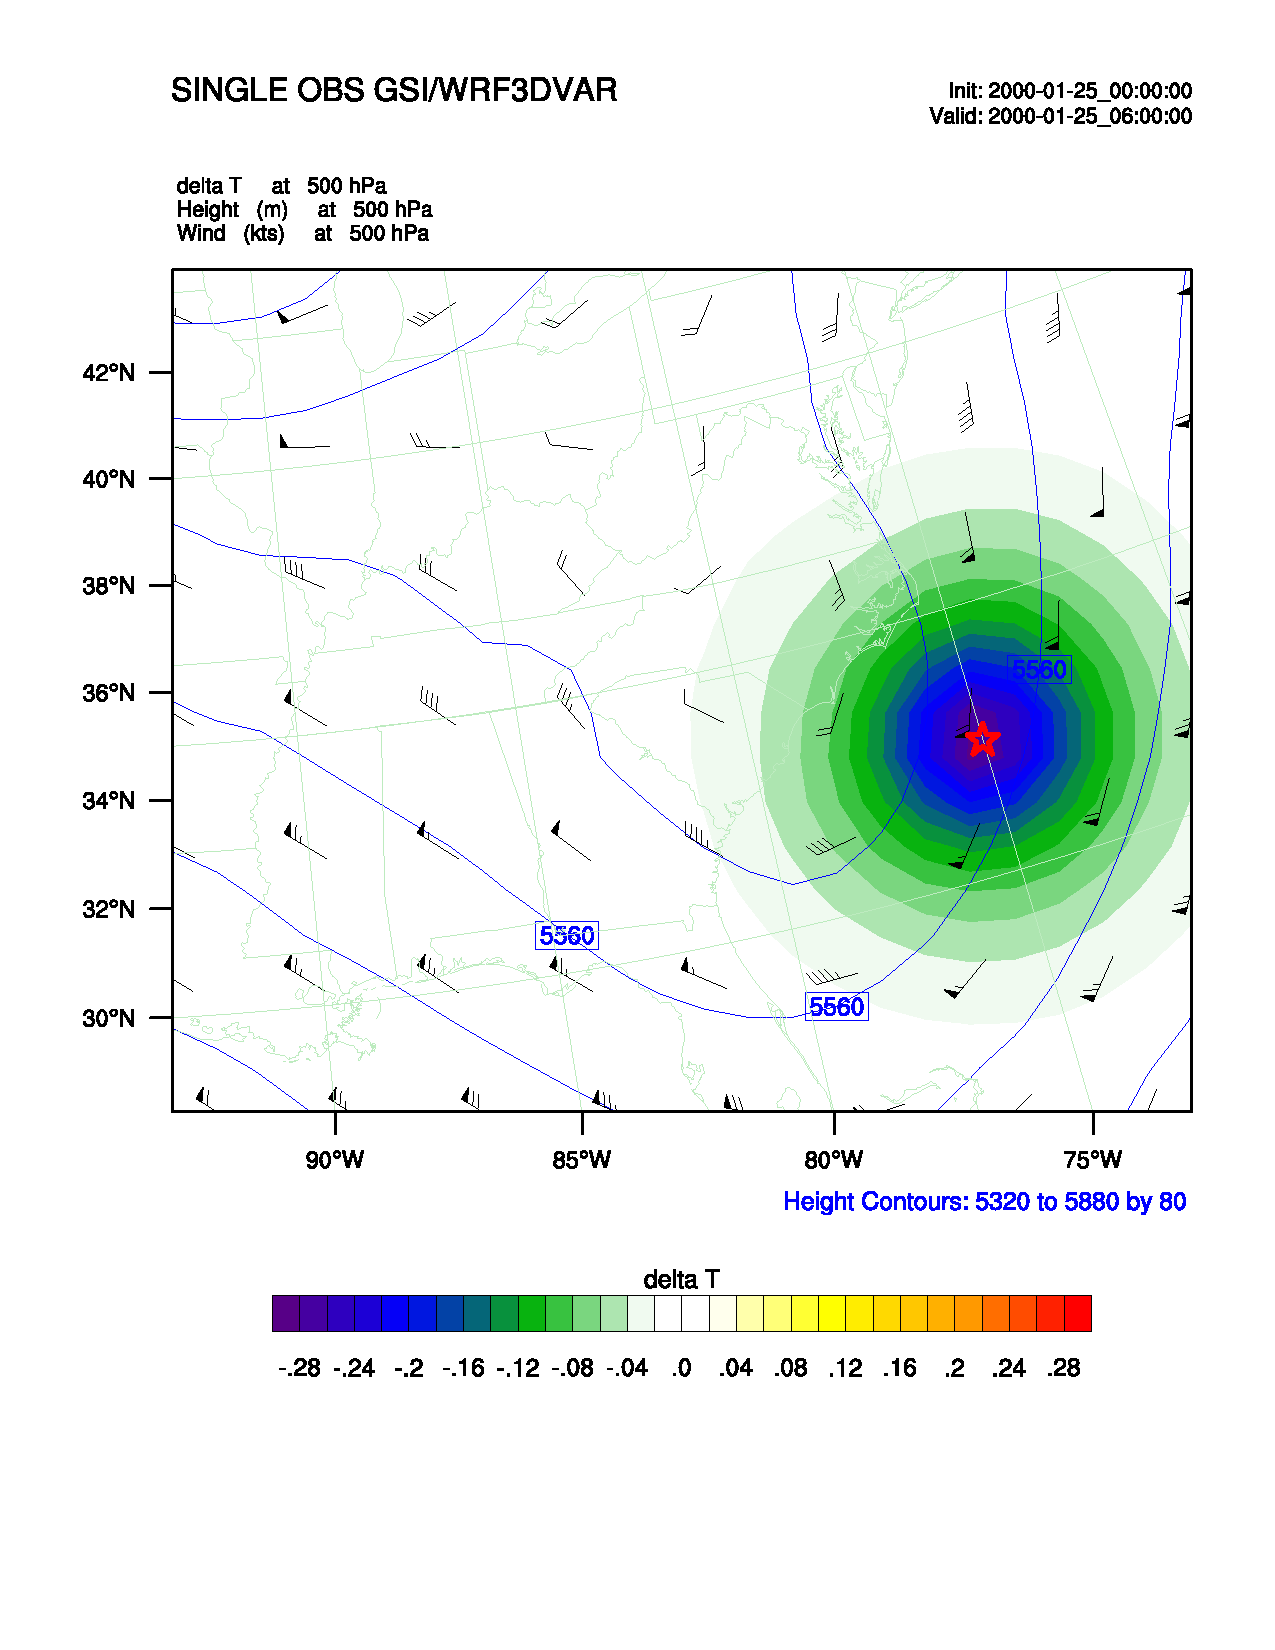
\includegraphics[scale=0.25, trim=10 5 10 10, clip]{gsi3dvar.pdf}
\end{tabular}
}
\end{comment}

\subsection{Tutorial case}

\begin{frame}[fragile]
\frametitle{\small Tutorial case -- Observation Usage}
\begin{center}
\includegraphics[scale=0.40, trim=25 200 50 150, clip]{obs_usage} 
\end{center}\pause
\begin{columns}[c]
\column{5cm}
\setbeamercolor{postit}{fg=black, bg=yellow}
\begin{beamerboxesrounded}[ lower=postit,shadow=true]{3DVAR}
{\tiny
\begin{verbatim}
   0:OBS_PARA: ps                       13842
   0:OBS_PARA: t                        20114
   0:OBS_PARA: q                        18743
   0:OBS_PARA: uv                       30894
   0:OBS_PARA: spd                         48
   0:OBS_PARA: sst                        503
   0:OBS_PARA: pw                         880
   ----------------Total--------------------
   47675
\end{verbatim}
}
\end{beamerboxesrounded}
\column{5cm}
\setbeamercolor{postit}{fg=black, bg=yellow}
\begin{beamerboxesrounded}[ lower=postit,shadow=true]{4DVAR}
{\tiny
\begin{verbatim}
   0:OBS_PARA: ps                       13585
   0:OBS_PARA: t                        20639
   0:OBS_PARA: q                        19180
   0:OBS_PARA: uv                       28802
   0:OBS_PARA: spd                         80
   0:OBS_PARA: sst                        494
   0:OBS_PARA: pw                         766
   ------------------------------
   0:OBS_PARA: ps                          10
   0:OBS_PARA: t                          552
   0:OBS_PARA: q                          490
   0:OBS_PARA: uv                         568
   ----------------Total-------------------
   45040
\end{verbatim}
}
\end{beamerboxesrounded}
\end{columns}
\end{frame}

\frame{
\frametitle{\small Cost functions and gradients --scaled by ALOG10}
\begin{tabular}{l r}
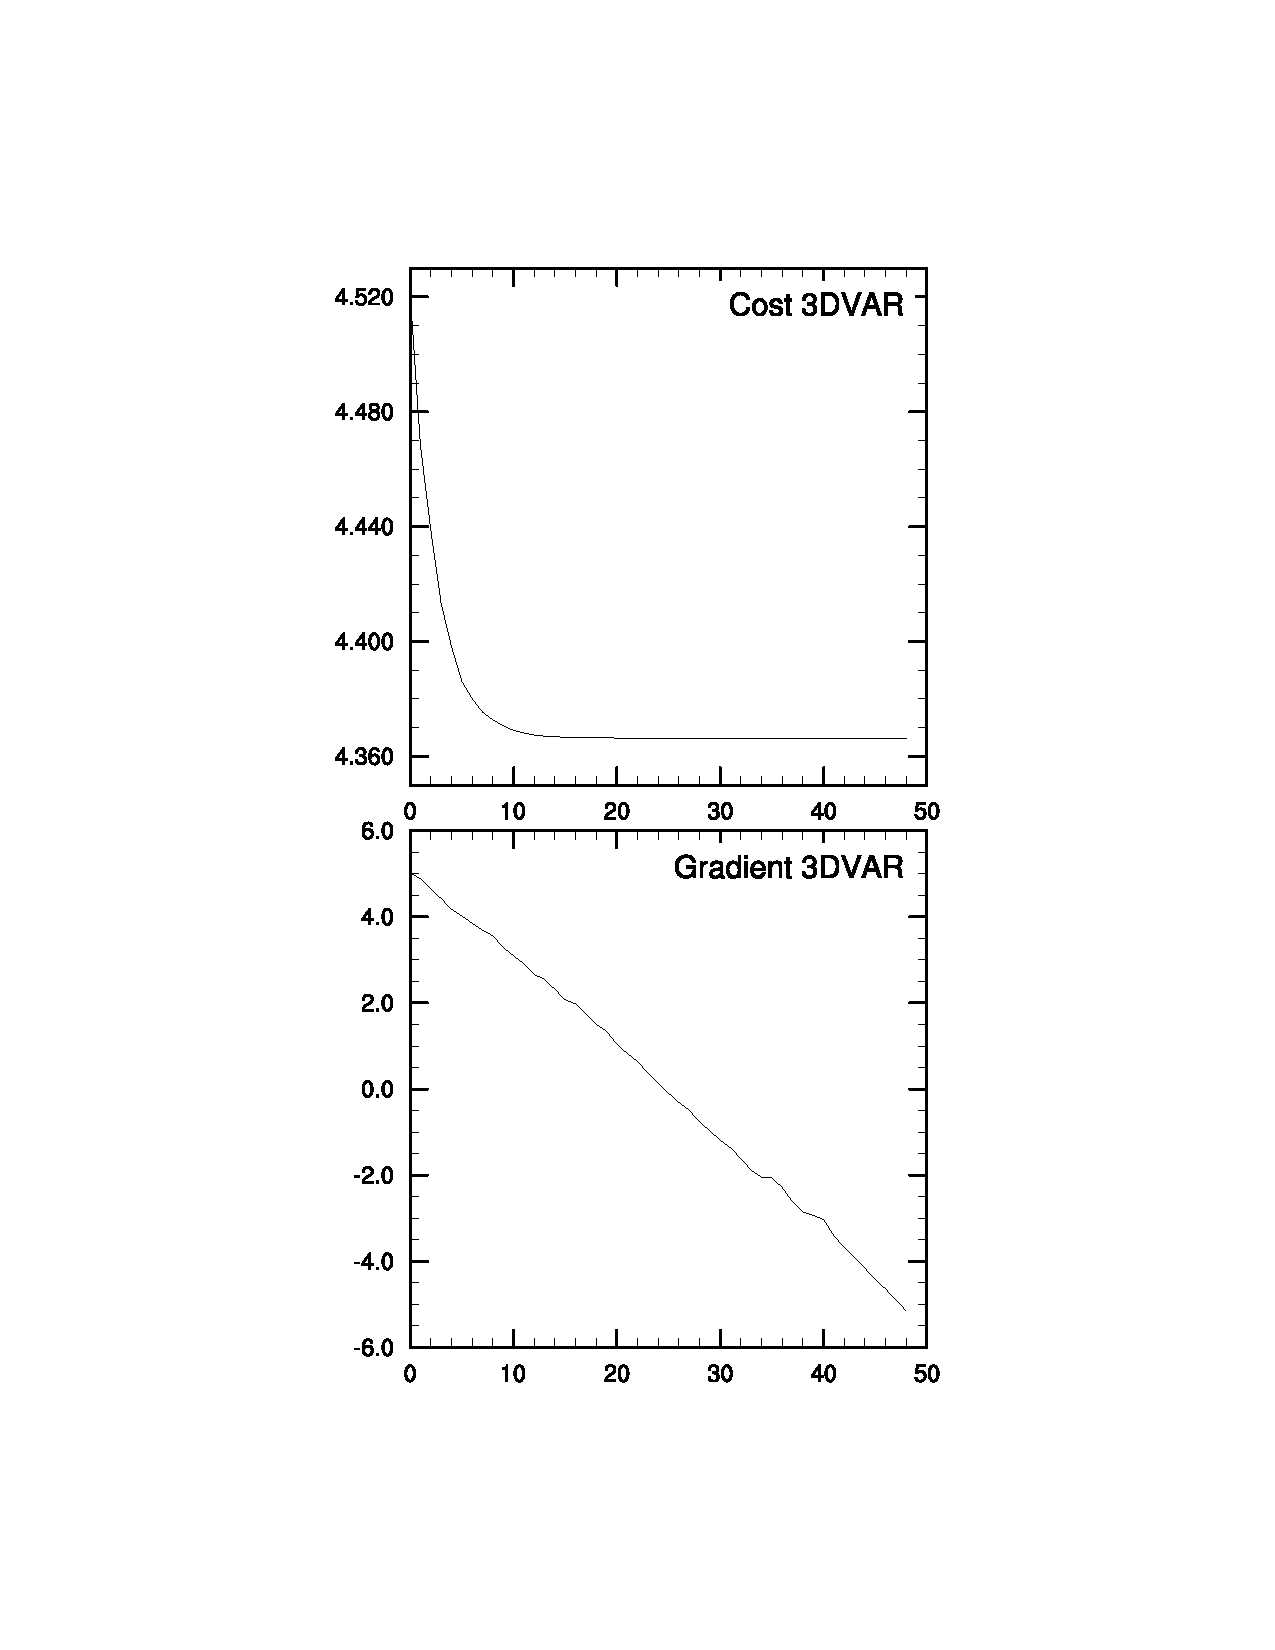
\includegraphics[scale=0.30, trim=10 5 100 50, clip]{3dvar_cost_grad.pdf} & 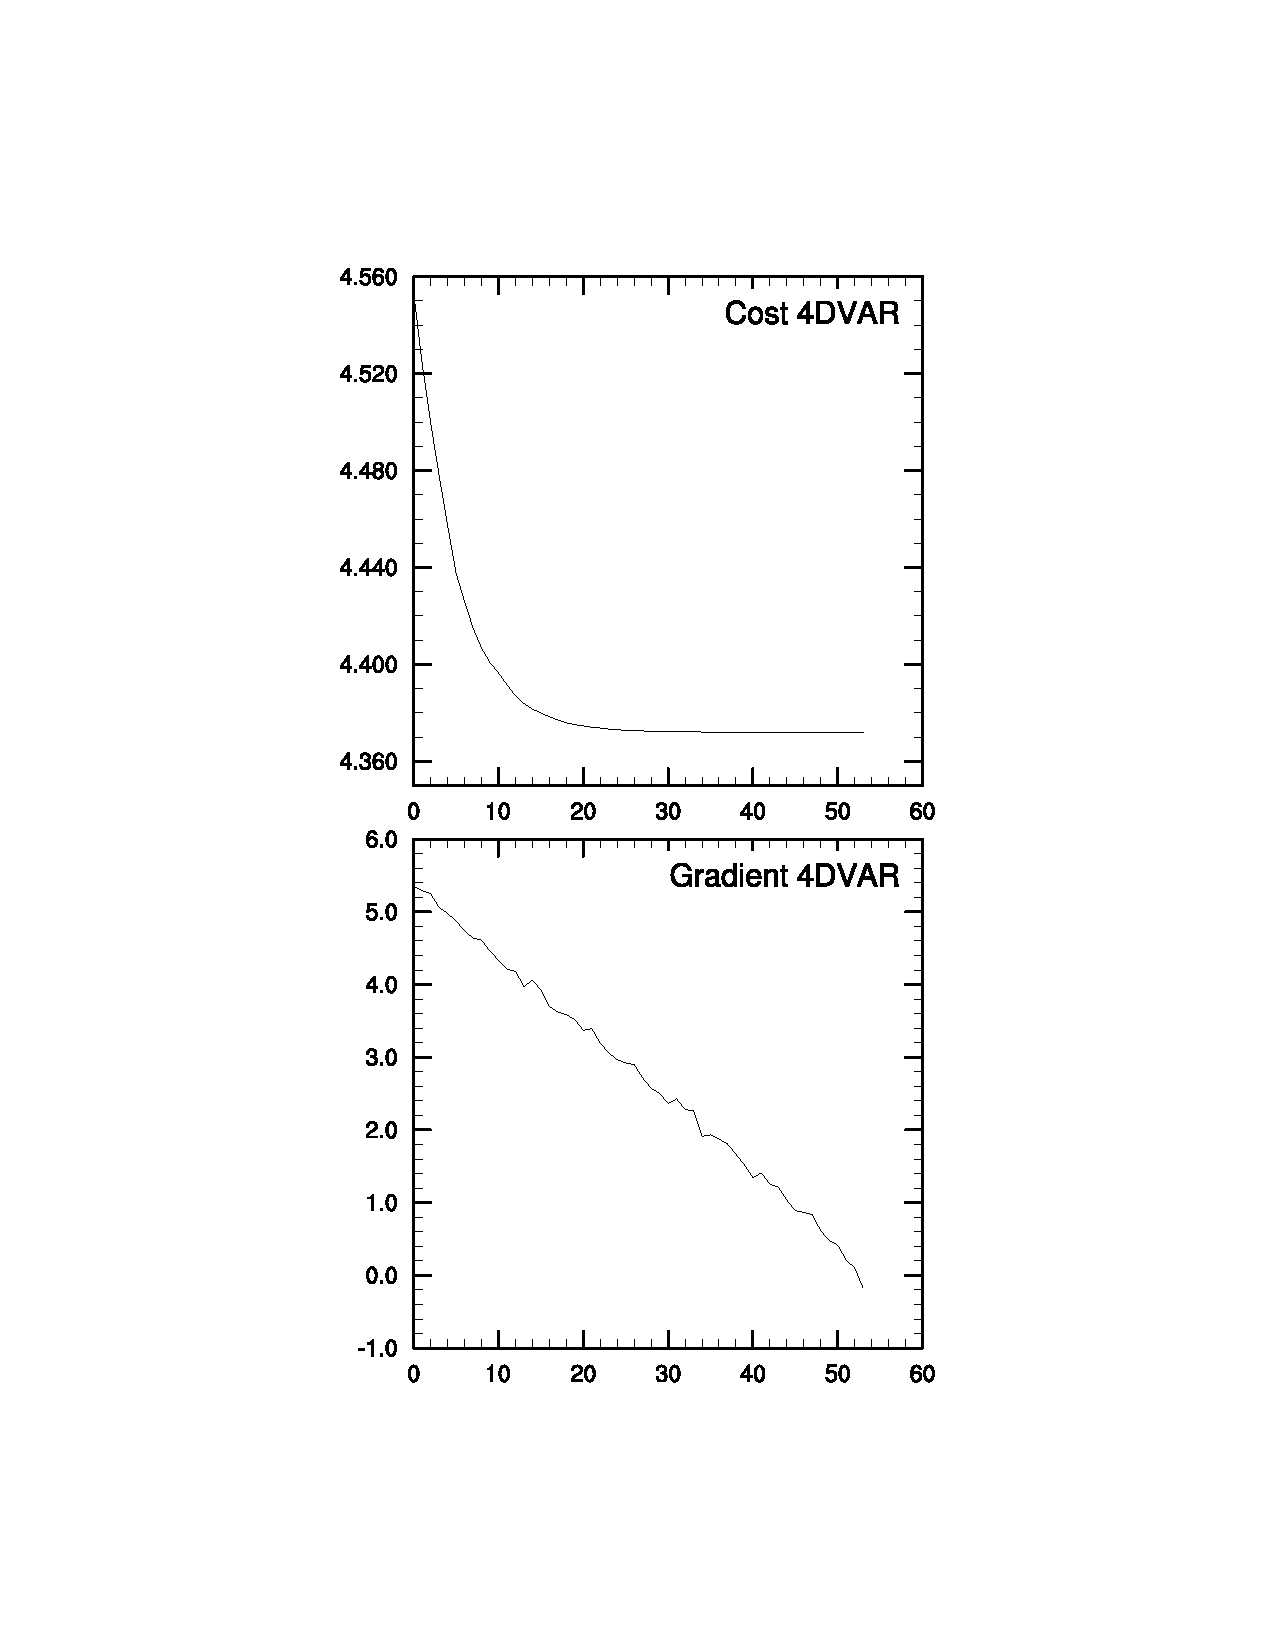
\includegraphics[scale=0.30, trim=150 5 10 50, clip]{4dvar_cost_grad.pdf}
\end{tabular}
}

\frame{
\frametitle{\small Sample increments comparison -- U, T}
\begin{tabular}{l r}
\includegraphics[scale=0.30, trim=50 230 100 250, clip]{3dvar_u_5_inc} & \includegraphics[scale=0.30, trim=100 230 100 250, clip]{3dvar_t_10_inc} \\
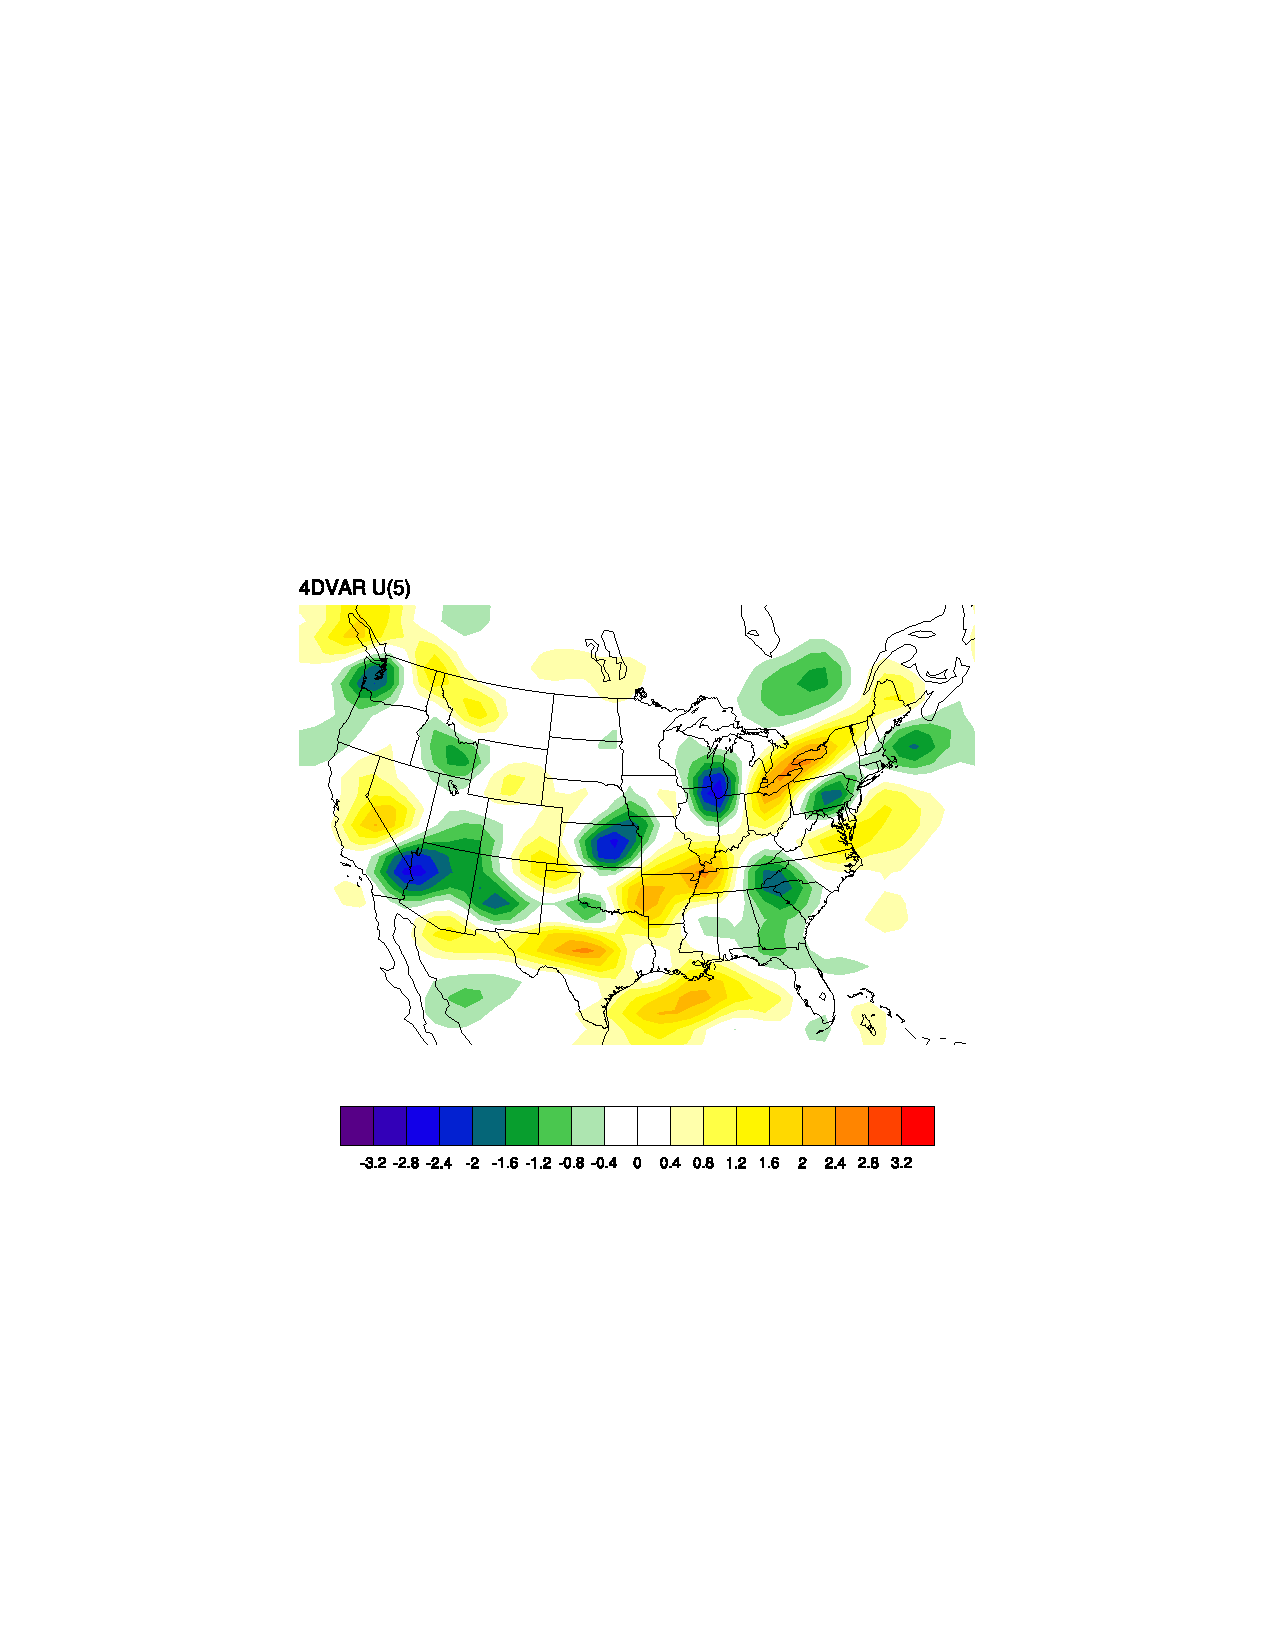
\includegraphics[scale=0.30, trim=50 160 100 250, clip]{4dvar_u_5_inc} & \includegraphics[scale=0.30, trim=100 160 100 250, clip]{4dvar_t_10_inc}
\end{tabular}
}

\frame{
\frametitle{\small Sample increments comparison -- MU, QVAPOR}
\begin{tabular}{l r}
\includegraphics[scale=0.30, trim=50 230 100 250, clip]{3dvar_mu_inc} & \includegraphics[scale=0.30, trim=100 230 100 250, clip]{3dvar_q_8_inc} \\
\includegraphics[scale=0.30, trim=50 160 100 250, clip]{4dvar_mu_inc} & \includegraphics[scale=0.30, trim=100 160 100 250, clip]{4dvar_q_8_inc}
\end{tabular}
}


\subsection{Real case}

\frame{
\frametitle{\small Domain}
\begin{itemize}
	\item \tiny{Grids: 105x72x28L}
	\item Resolution: 60km
	\item Period: 2010091100-2010092600 @0Z,6Z,12Z,18Z
	\item First guess is the 12h forecast from NCEP FNL
	\item 48h forecasts from FG, 3DVAR and 4DVAR
	\item Verified against NCEP GDAS prepbufr data, done by NCAR MET
\end{itemize}
\begin{center}
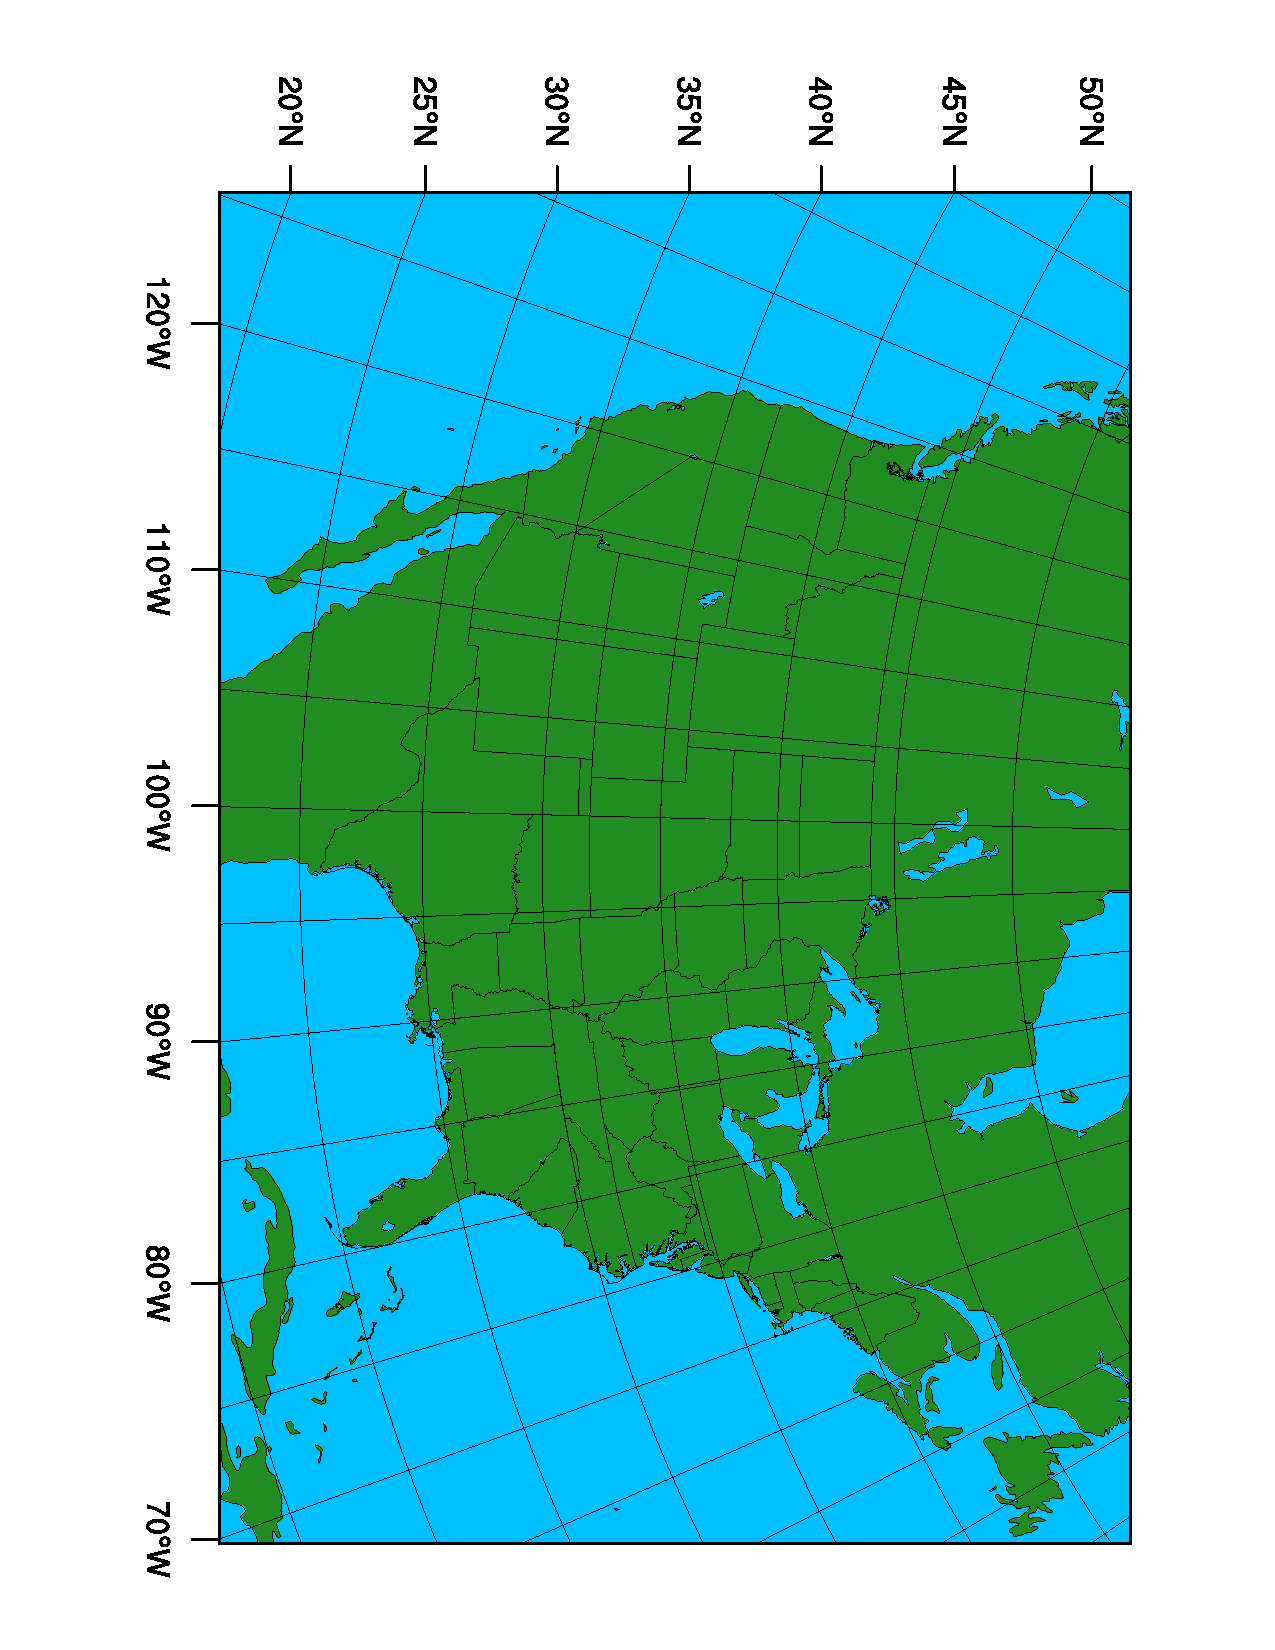
\includegraphics[scale=0.25, trim=0 0 50 0, clip, angle=90]{domain.pdf} 
\end{center}
}

\frame{
\frametitle{\small Averaged RMSE of surface forecasts}
\begin{center}
%\includegraphics[scale=0.27, trim=0 100 0 60, clip]{Bias_surface_all_var.pdf}
\includegraphics[scale=0.30, trim=0 100 0 60, clip]{RMSE_surface_all_var.pdf}
\end{center}
}

\frame{
\frametitle{\small Averaged RMSE of upper level U component}
\begin{center}
%\includegraphics[scale=0.27, trim=0 100 0 60, clip]{Bias_upplevel_UGRD.pdf}
\includegraphics[scale=0.30, trim=0 90 0 60, clip]{RMSE_upplevel_UGRD.pdf}
\end{center}
}

\frame{
\frametitle{\small Averaged RMSE of upper level V component}
\begin{center}
%\includegraphics[scale=0.27, trim=0 100 0 60, clip]{Bias_upplevel_VGRD.pdf}%
\includegraphics[scale=0.30, trim=0 95 0 60, clip]{RMSE_upplevel_VGRD.pdf}
\end{center}
}

\frame{
\frametitle{\small Averaged RMSE of upper level Temperature}
\begin{center}
%\includegraphics[scale=0.27, trim=0 100 0 60, clip]{Bias_upplevel_TMP.pdf}
\includegraphics[scale=0.30, trim=0 90 0 60, clip]{RMSE_upplevel_TMP.pdf}
\end{center}
}

\frame{
\frametitle{\small Averaged RMSE of upper level Moisture}
\begin{center}
%\includegraphics[scale=0.27, trim=0 100 0 60, clip]{Bias_upplevel_SPFH.pdf}
\includegraphics[scale=0.30, trim=0 90 0 60, clip]{RMSE_upplevel_SPFH.pdf}
\end{center}
}


%%%%%%%%%%%%%%%%%%%%%%%%%%%%%%%%%
\subsection{Summary}

\frame{
\frametitle{\small Summary}
\begin{itemize}
	\item The basic GSI/WRF 4DVAR system was developed with minimum codes modification. \pause
	\item The single observation exp. preliminarily confirm that the system is valid and is able to produce flow dependent increments. \pause
	%\item The increments produced by 4DVAR run with tutorial case are comparable with the 3DVAR run.\pause
	\item The real case shows the desirable performance of 4DVAR.
\end{itemize}
}

\frame{
\frametitle{\small Under development}
\begin{itemize}
	\item Add simplified physics packages into WRFPLUS: surface drag(\alert{done}), large scale condensation(\alert{done}), a simplified cumulus scheme(\alert{done}), as well as a radiation scheme. \pause
	\item Parallelization of WRF tangent linear codes (\alert{done}) \pause
	\item Parallelization of WRF adjoint codes. \pause
	\item The observation processing for 4DVAR mode is still a black box for us, need to be investigated. \pause
	\item Adjoint check achieved 5-digital identical, need to debug the code to find the bugs. \pause
	\item Multiple outer loops for 4DVAR. \pause
	\item Assimilation of radiance data. \pause
	\item Adapt gradient check for GSI-based WRF 4DVAR. \pause
	\item Adapt digital filter as a weak constrain for GSI-based WRF 4DVAR.
\end{itemize}
}


%%%%%%%%%%%%%%%%%%%%%%%%%%%%%%%%%%%
\fst{}{
\begin{center}
~\\
~\\
~\\
~\\
~\\
{\huge{\color{red}Thank You}}\\
~\\
~\\
~\\
~\\
~\\
{\tiny{\color{blue}The NESL Mission is: \\
To advance understanding of weather, climate, atmospheric composition and processes;\\
To provide facility support to the wider community; and, \\
To apply the results to benefit society.\\}}
~\\
{\small{NCAR is sponsored by the National Science Foundation}}
\end{center}
}

\end{document}
